\chapter{Loading data from other databases into the EFABIS }

\newpage 
\section{Objectives}
Various countries over the Europe have now running databases. These 
databases run on different operating systems and database engines. 
A general procedure has to be developed for these countries in case their want to share they data with EFABIS database.
This procedure should be as simple as possible and 
easy repeatable, independent from database engine and 
operating system. \\
This procedure should be done by person without any special knowledge about 
computer programming etc. All data should be prepared and validated on country 
side.\section{Side conditions/Requirements}
On the EFABIS side we need to have one program which will be able to load data 
from different NON EFABIS databases. Responsibility for NON EFABIS data is on 
data owner. Data which other countries want to load into EFABIS 
data have to be in English for EFABIS. 
Translation from national to English language will be done on the country 
side.\section{Design proposal}
\subsection{EFABIS side needs to}
\begin{itemize}
\item share EFABIS database structure 
\item share core parts i.e.: colours, mainuse etc.
\item create data stream templates
\item generate templates based on database model - FAO, EAAP, National
\item receive data from country side
\item load all data into EFABIS database with one piece of software
\item define the validation rules and constrains
\end{itemize}

\subsection{Country side needs to}
\begin{itemize}
\item receive EFABIS database structure in templates to fill in core parts of EFABIS database
\item create data stream files
\item validate data
\item transfer data to EFABIS side
\end{itemize}

\subsection{Mapping database}
Before start data exporting from source database, mapping of data must be done.
EFABIS database structure will be available for country. EFABIS database structure will be extended during mapping process with information about country database.

\subsection{Creating transfer files}
Country receive templates of data stream files to fill. 

\subsection{Data translation and validation}
Data validation must be done on country side. Validation should also cover measurements unit conversion if country use different measurements unit than defined in EFABIS database. Country also must make translation of data from country language into official language.

\subsection{Transfer files to EFABIS side}
Country must transfer only valid data. Data have to be transferred to the EFABIS side in electronic form.
For data transmission standard method should be used (FTP, SCP etc.)

\subsection{Loading into EFABIS database}
After transmission data will be loaded into EFABIS database. Loading process will be the same for data from all countries. Standard load objects will be used for loading data for countries.

\subsection{Statistics}
When loading process is finished, statistic about loaded data will be generated and send to country via e-mail if available.
Status of loading process will be available on the Internet for the country.


\newpage 
\section{Implementation}


\subsection{Implementation - general}

To share important data with country, standard method must be available. This method must work with most databases and operating systems. EFABIS side uses Perl scripts to create templates and for data loading. Database structure of EFABIS database will be shared as XML file. For data-stream files (data exchange) CSV - Comma Separated Value file format will be used. Country side has to have some utility to dump database structure into XML file. The structure of the database can be also written manually into XML file using EFABIS DTD files for data types etc. 

\begin{landscape}
\subsection{Important steps to do}

\begin{tabular}{|p{0,5 cm}|p{2,5 cm}|p{2,5 cm}|p{6 cm}|p{2,5 cm}|}
\hline Step& Description & Implementation &  	Comments & Responsibility\\ 
\hline  1&  Preparing XML files for the country& relatively easy    & This step can be made automatically (See \ref{sub:coredata})&EFABIS side\\ 
\hline  2&  Mapping database & relatively easy	 & Step easy for implementation, but requires manual work to map fields and database content (See \ref{sub:mapping})&country side\\ 
\hline  3&  Data exporting& difficult & This step depends strongly on the mapping step. If our mapping file is very complicated (many fields) this piece of software must be very robust to keep data in correct order.(See \ref{sub:exportdata})&country side \\ 
\hline  4&   Data translation&  relatively easy& This part of software should extract text data from all exported data (i.e. by field type) and make it available for translation and future loading into EFABIS database (See \ref{sub:translatedata})&country side\\ 
\hline	5& Data validation& difficult& Data validation according to defined validation rules(See \ref{sub:validdata})&country side\\
\hline  6& Transfer and loading country data	 & half done & When data will be available (after mapping, exporting, translation and validation), it can be loaded into EFABIS database (See \ref{sub:loaddata})&EFABIS and country\\ 
\hline	7& Creating statistics & relatively easy & Create report about loading process and send it to the country (See \ref{sub:createstat})&EFABIS side\\
\hline 
\end{tabular}
\end{landscape}

\subsection{Preparing core data - EFABIS side}
 \label{sub:coredata}

\textbf{Inputs}:
\begin{enumerate}
\item EFABIS database XML model
\item connection to EFABIS database
\end{enumerate}
\textbf{Outputs}:
\begin{enumerate}
\item EFABIS XML files (templates)
\end{enumerate}
\textbf{Description}:\\
Database structure of EFABIS database is available as XML file. Three levels of database are defined: FAO (global level), EAAP (regional level) and NATIONAL (country level). This utility has to be able to read database structure from file and database content from database back-end. If all information will be available, XML file templates will be created. This file will contain information about database structure and core data of EFABIS database i.e. colours, main-use, mcname etc. The countries needs this information to create mapping (structure and data) and correctly export data.
 For application schema see figure \ref{fig:schema1}.\\
\begin{figure}[h]
\begin{center}
   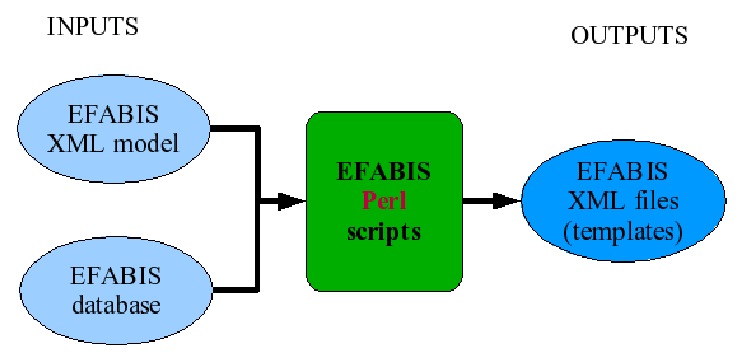
\includegraphics{/home/zgr/soltys/devel/apiis/doc/developer/loading_from_other_db/schema1b.eps}
   \caption{Data preparation schema}
   \label{fig:schema1}
\end{center}
\end{figure}
\\Part of EFABIS structure in XML file which will be shared with country:\\
\scriptsize {
\begin{verbatim}
<table DB_LEVEL="FAO" name="breeds_horns">
        <column CHECK="NotNull ,ForeignKey breeds breed_id" DATA=""
            DATATYPE="BIGINT" DB_LEVEL="FAO" DEFAULT=""
            DESCRIPTION="breed id" ERROR="" LENGTH="20" MODIFY="" name="breed_id"/>
        <column CHECK="List 0 2 4 0/2 0/2/4 0/4 2/4" DATATYPE="CHAR"
            DB_LEVEL="FAO" DESCRIPTION="number of horns (males)"
            LENGTH="20" name="male"/>
        <column CHECK="List 0 2 4 0/2 0/2/4 0/4 2/4" DATATYPE="CHAR"
            DB_LEVEL="FAO" DESCRIPTION="number of horns (females)"
            LENGTH="20" name="female"/>
        <TABLE>
            <CONSTRAINTS INDEX="unique breed_id, unique guid"/>
        </TABLE>
</table>

\end{verbatim}}
\normalsize
\subsection{Mapping database structure and data - country side}
\label{sub:mapping}
\textbf{Inputs}:
\begin{enumerate}
\item EFABIS XML files (templates)
\item connection to country database or country database model
\end{enumerate}
\textbf{Outputs}:
\begin{enumerate}
\item country XML map file
\end{enumerate}
\textbf{Description}:\\
Mapping is most important step in the process of data transfer from country database into EFABIS database.
In this step  database structure mapping and data mapping have to be done. Database structure mapping means that for all fields in EFABIS database we should choose corresponding field in country database, create link between these fields. Country database have different structure than EFABIS database. Country also use different foreign keys definition and different relations between tables. \\
To start, mapping process needs to have EFABIS XML files (templates) and connection to country database or country database model available as XML file. Country database structure can be read from file or from country database through i.e ODBC ( \textbf{O}pen  \textbf{D}ata \textbf{B}ase \textbf{C}onnectivity ) connection. Through ODBC connection only table names, column names and types without relation between tables (foreign keys relations) can be read from database. This missing relations must be defined in mapping process manually. Mapping process will take long time according to number of fields which must be mapped. EFABIS database contain i.e. about  \textbf{1000 different fields}, French database about \textbf{1400 different fields}. If one type of information is only in one table mapping process will be not very difficult. Some countries are using database for several years and database structure was sometimes modified during years of use. In most of cases it means that information on country side is not only on one place (one table) but in several tables. This makes mapping process more difficult.\\
Lets assume that country have some utility for mapping with GUI interface. Table names and column names are represented there as drop down list. We have also some check fields to indicate FK relations etc. Person which is creating mapping just need to choose from menu field for EFABIS at one side, and then corresponding field on the country side. Then indicate if it is value or just foreign key to some value in other place.  If we need i.e 15 seconds to choose correct value from the drop down list, than we will need at least 1 minute for each field (choose EFABIS table, choose EFABIS field, choose coutry side table, choose country side field). According to numbers of fields, it will take al least 25 hours just for structure mapping.\\
Part of database structure file after mapping process:\\
\scriptsize {
\begin{verbatim}
<table DB_LEVEL="FAO" name="breeds_horns">
        <column CHECK="NotNull ,ForeignKey breeds breed_id" DATA=""
            DATATYPE="BIGINT" DB_LEVEL="FAO" DEFAULT=""
            DESCRIPTION="breed id" ERROR="" LENGTH="20" MODIFY="" name="breed_id" 
	    src_column="CodeRace" src_table="RaceAnnee"/>
        <column CHECK="List 0 2 4 0/2 0/2/4 0/4 2/4" DATATYPE="CHAR"
            DB_LEVEL="FAO" DESCRIPTION="number of horns (males)"
            LENGTH="20" name="male"
	    src_column="field 1" src_table="table 1" />
        <column CHECK="List 0 2 4 0/2 0/2/4 0/4 2/4" DATATYPE="CHAR"
            DB_LEVEL="FAO" DESCRIPTION="number of horns (females)"
            LENGTH="20" name="female"
	    src_column="field 2" src_table="table 2" />
        <TABLE>
            <CONSTRAINTS INDEX="unique breed_id, unique guid"/>
        </TABLE>
</table>

\end{verbatim}}
\normalsize
After structure mapping is done, next step can be started. In this step, links between all foreign key entries must be created. All foreign key entries from country database must be mapped into corresponding values on the EFABIS side i.e colours, sex, main-use etc. This process must be done mostly manually, software addition here can only save this links between values and write it into file (i.e. XML file) for future use in data exporting step.\\
 Data mapping will be also difficult. There are different foreign keys in both databases i.e in EFABIS database there is more that 100 basic foreign keys entries mapping only for colours, main-use etc. In French database there is about 200 basic values which should be linked to EFABIS values.\\
Data mapping process will take i.e approximately 1 minute for each field. If we have about 300 fields it means we need at least 5 hours to do this.
The country data are not in official language during mapping process. In this step some basic translations (code conversions) must be done. Country values in country language can be mapped into EFABIS official language values. It may happen that country has more or less values to describe something i.e. sex . The person who will make this mapping have to know what to do then.
Output from mapping process is EFABIS database structure extended with information about country database - country XML map file. \\
\textbf{Summary}:\\
For this step must have (or develop) utility for mapping process and person which can make mapping.\\
\begin{figure}
   \centering
   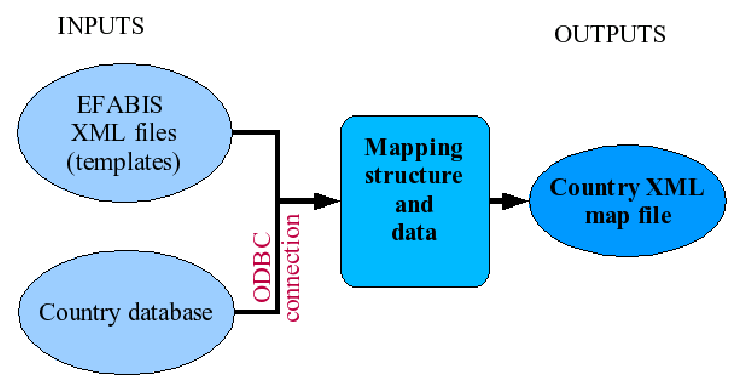
\includegraphics{./loading_from_other_db/schema2b.eps}
   \caption{Data mapping schema}
   \label{fig:schema2}
\end{figure}
\begin{figure}
   \centering
   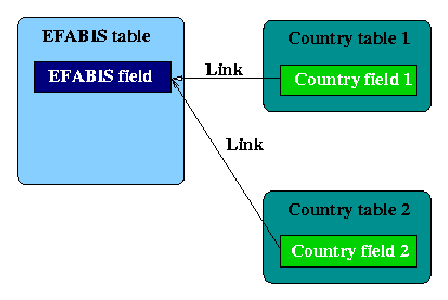
\includegraphics{./loading_from_other_db/map_ex1.eps}
   \caption{Example of structure mapping}
   \label{fig:map_ex1}
\end{figure}
%\begin{figure}
%   \centering
%   \includegraphics{map_ex2.png}
%   \caption{Example of data mapping}
%   \label{fig:map_ex2}
%\end{figure}

\subsection{Data exporting - country side}
\label{sub:exportdata}
\textbf{Inputs}:
\begin{enumerate}
\item country XML map file
\item connection to country database
\end{enumerate}
\textbf{Outputs}:
\begin{enumerate}
\item data in country language
\end{enumerate}
\textbf{Description}:\\
Before start exporting country data from database, mapping process must be finished. Country XML map file must be available. Country has to developed some utility which can read XML map file and according to defined their relations create SQL statements. These statements should be able to get correct data from database. Statement may be executed via ODBC connection or other database programming environment related to used database engine. Results of these statements have to be written into templates files with defined structure.

\subsection{Data translation - country side}
\label{sub:translatedata}
\textbf{Inputs}:
\begin{enumerate}
\item data in country language
\end{enumerate}
\textbf{Outputs}:
\begin{enumerate}
\item data for validation
\end{enumerate}
\textbf{Description}:\\
After data are exported from database, text fields need to be extracted from data and translation process should be done. Data for translation will be put into text file which then translator can get and translate. Translated information in same format will be than again put into correct place in data files. For numeric data measurement unit conversion must be done. 
\begin{figure}[ht]
   \centering
   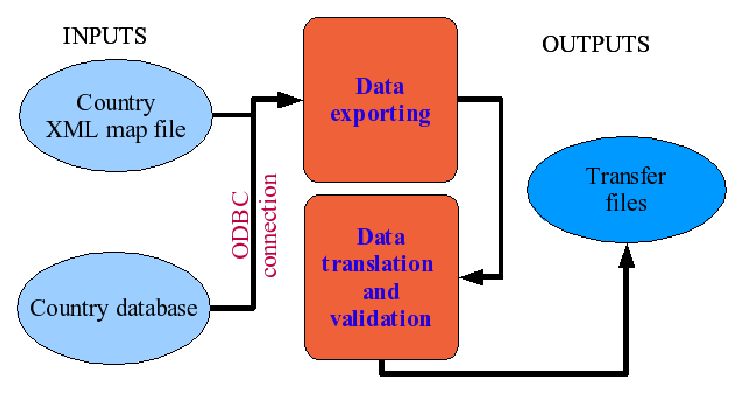
\includegraphics{./loading_from_other_db/schema3b.eps}
   \caption{Data exporting, translation and validation schema}
   \label{fig:schema3}
\end{figure}
\subsection{Data validation - country side}
\label{sub:validdata}
\textbf{Inputs}:
\begin{enumerate}
\item data for validation
\end{enumerate}
\textbf{Outputs}:
\begin{enumerate}
\item transfer files
\end{enumerate}
\textbf{Description}:\\
Validation of data must be done on country side. Country is responsible for data and only country know if data are correct or not. After validation process valid data are expected on the EFABIS side.


\subsection{Loading country data - EFABIS side}
\label{sub:loaddata}
\begin{figure}[h]
\vspace{1cm}
   \centering
   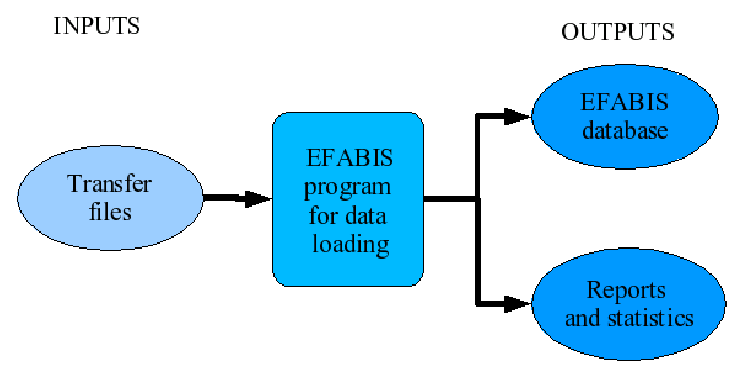
\includegraphics{./loading_from_other_db/schema4b.eps}
   \caption{Data loading into EFABIS database schema}
   \label{fig:schema4}\vspace{1cm}
\end{figure}
\textbf{Inputs}:
\begin{enumerate}
\item transfer files
\end{enumerate}
\textbf{Outputs}:
\begin{enumerate}
\item loaded country data
\end{enumerate}
\textbf{Description}:\\
Data received from country have to be prepared in defined form. Country must send files created in data exporting step. Data have to be translated into official language and validated according to validation rules. Only valid data will be loaded into EFABIS database.


\subsection{Creating statistics}
\label{sub:createstat}
\textbf{Inputs}:
\begin{enumerate}
\item loaded country data
\end{enumerate}
\textbf{Outputs}:
\begin{enumerate}
\item report
\end{enumerate}
\textbf{Description}:\\
Statistics will be available online on the Internet during all loading process for countries. Data for creating statistics will be store in EFABIS database. When data loading will be finished, report for country will be created and send to responsible person in country via e-mail if available.

\newpage
\makeatother
\section{Summary}
Process of loading data from NON EFABIS database to the EFABIS database is very complicated procedure. It requires many manual work.\\
Probably each country has their own database structure. It means that each country has to create map file for their database, go through hundreds fields and many foreign keys. Every time country needs to prepare also translation of text fields (descriptions etc.) If the country change database structure, it needs again to recreate map file, and to create core data mapping. At least the country need to check all fields mapping, export data, translate data, validate etc. The data translation is most difficult, because text data must be extracted from database and than prepared for translator, after translation need to be placed again to transfer files. Data can not be automatically translated at this time. Process shown in this paper can be used for data exchange relatively easy with some limitations, i.e. limit only for numeric populations data.
 \\The table below shows short summary for implementation difficulty (Implementation difficulty / time) and manual working time which country needs in each step (Manual working time).\\ \\
%\begin{landscape}
\begin{tabular}{|p{0,5 cm}|p{3,5 cm}|p{3 cm}|p{3,5 cm}|}
\hline Step & Description &Implementation difficulty / time

& Manual working time \\ 
\hline  1 & Preparing XML files for the country (See: \ref{sub:coredata})& relatively easy / short    &  less than 1 hour\\ 
\hline  2 & Mapping database (See: \ref{sub:mapping}) & relatively easy / not too long & manual work choosing source and target fields / at least 30 hours \\ 
\hline  3 & Data exporting (See: \ref{sub:exportdata})& difficult / long & manual check SQL statements / depends on  amount of data \\ 
\hline  4 & Data translation (See: \ref{sub:translatedata})&  relatively easy / short & manual translation of extracted text fields / approximately 2h per page A4  \\ 
\hline	5 & Data validation (See: \ref{sub:validdata})& difficult / long& depends on data amount / ???\\
\hline  6 & Transfer and loading country data (See: \ref{sub:loaddata})	 & half done / short & depends on amount of data\\ 
\hline	7 & Creating statistics (See: \ref{sub:createstat})& relatively easy / short & short\\
%\hline    & Total: &  & \\
\hline 
\end{tabular}
%\end{landscape}

\end{document}
